\documentclass[pagesize,DIV=calc,12pt,draft]{scrreprt}
\usepackage[plain]{fullpage}
\usepackage[utf8]{inputenc}
\usepackage[T1]{fontenc}
\usepackage[ngerman]{babel}
\usepackage{amsmath}
\usepackage{amsfonts}
\usepackage{amssymb}
\usepackage{graphicx}
\usepackage[normal,it,footnotesize]{caption}
\usepackage{booktabs}
\usepackage[table]{xcolor}
\usepackage{listings}
\usepackage{paralist}
\usepackage{textgreek}

\usepackage[breaklinks]{hyperref}
\hypersetup{
 colorlinks,%
 citecolor=black,%
 filecolor=black,%
 linkcolor=black,%
 urlcolor=hhublau,%
 hypertexnames=false
 }

% FARBEN

\definecolor{hhublau}{rgb}{0.09,0.435,0.757}

% TikZ

\usepackage{tikz}
\usetikzlibrary{positioning,chains,fit,shapes}

% ZEILENABSTAND

\usepackage{setspace}
\onehalfspacing

\usepackage{lmodern}

% VERSCHIEDENES

\setcounter{secnumdepth}{-1}

%%%%%%%%%%%%%%%%%%%%%%%%%%%%%%%%%%%%%%%%%%%%%%%%%%%%%%%%%%%%%%%%%%%%%%%%%%%%%%%%
%%%%%%%%%%%%%%%%%%%%%%%%%%%%%%%%%%%%%%%%%%%%%%%%%%%%%%%%%%%%%%%%%%%%%%%%%%%%%%%%

\begin{document}

\lstloadlanguages{SQL,bash}
\lstset{
	literate= {Ö}{{\"O}}1 {Ä}{{\"A}}1 {Ü}{{\"U}}1 {ß}{{\ss}}2
	 {ü}{{\"u}}1 {ä}{{\"a}}1 {ö}{{\"o}}1,
	numbers=left,
	basicstyle=\footnotesize,
	showstringspaces=false,
	inputencoding=utf8,
	extendedchars=true,
	breaklines=true,
	breakindent=0pt,
}

\chapter{Einführungsteil}

\section{A multilingual Dictionary of Ophthalmology (Aufbau und Umfang des Dictionarys, was bisher daran gemacht wurde)}

Ausgangspunkt dieser Arbeit ist das \href{http://www.zeitzfrankozeitz.de/index.php/fachwoerterbuch.html}{digitale multilinguale Wörterbuch der Augenheilkunde} des Augenarztes Dr. 
Philipp Franko Zeitz, das seit 2010 existiert und online auf der Webpräsenz der Düsseldorfer Augenklinik Zeitz Franko Zeitz zugänglich ist. Das Wörterbuch umfasst mittlerweile fast 25.000 händisch gepflegte Einträge aus dem Bereich der Augenheilkunde in 13 (anfänglich 8) Sprachen. 
Einträge enthalten Erklärungen, Abkürzungen, sowie Übersetzungs- und Synonymverweise, welche mittels eines simplen Suchformulars gefunden werden können. 
Seit 2011 sind sowohl die Funktionen, als auch der Inhalt des Wörterbuchs stetig erweitert worden, was ein weitreichendes Interesse am Wörterbuch mit sich zog - auch im internationalen Raum. 
Ergebnisse sind neben der nun breiten Sprachunterstützung eine benutzerfreundliche Schnittstelle mit verbesserten Suchfunktionen und ein Bildatlas mit annähernd 2000 Bildern, die vereinzelte Einträge illustrieren. Die Einträge des Wörterbuchs verteilten sich zum Zeitpunkt des Projektbeginns auf ca. 2500 Konzepte, die jeweils unterschiedliche Ausprägungen eines medizinischen Begriffs zusammenfassen (also alle Einträge des Wörterbuchs mit jeweils derselben Bedeutung, wie Synonyme, Übersetzungen und unterschiedliche Schreibweisen desselben Begriffs). 
In Anlehnung an den bekannten englischsprachigen Thesaurus WordNet werden diese Konzepte - bzw. 
Mengen an synonymen Termen - im Nachfolgenden \emph{Synsets} genannt. 
Synsets werden im Wörterbuch intern durch eine eindeutige Kennziffer ausgezeichnet, die das Identifizieren von Bedeutungen sehr einfach macht und damit einen sehr guten Ansatz zum Ausbau der Bedeutungstruktur innerhalb des Wörterbuchs liefert.

\section{Ideen und Zielsetzung (SimuLLda, Formale Begriffsanalyse, lexical gap)}

Ziel des nachfolgend vorgestellten Teamprojekts war es, die Einträge des \emph{Wörterbuchs der Augenheilkunde} zu erweitern um ihre jeweilige Repräsentation als formalen Begriff. 
Die Synsets des Wörterbuchs bilden im Sinne der Formalen Begriffsanalyse, die nachfolgend einführend erläutert wird, die Menge an Objekten. 
Um diese Objekte repräsentieren zu können werden sie beschreibende Merkmale benötigt. 
Die Erweiterung des Wörterbuchs beschäftigt sich also vornehmlich mit der Frage, wie diese Merkmale erzeugt und den entsprechenden Objekten, den Synsets, zugewiesen werden. 
Hierzu bieten sich Methoden der Informationsextraktion an, die im Hauptteil der Arbeit erläutert werden. 
Bezüglich der Abdeckung an Synsets im Wörterbuch sind für jede der berücksichtigten Sprachen unterschiedliche Anteile erkennbar. 
Ein Grund dafür könnte unzureichendes Quellenmaterial bei der Erstellung des Wörterbuchs gewesen sein. 
Ein anderer Grund könnte sein, dass es bestimmte Begriffe in der einen Sprache gibt und in anderen Sprachen nicht. 
Einträge mittels formaler Begriffe auszudrücken und damit über deren Merkmale prinzipiell übersetzbar zu machen in Sprachen, in denen es die Bezeichnung nicht gibt, ist eine Idee, die auf die Arbeit von Janssen, 2002 zurückgeht. 
Solcherlei Lücken, lexical gaps genannt, gibt es im Wörterbuch der Augenheilkunde ebenfalls. 
Dieses Phänomen kann umso ausgeprägter werden, je spezifischer die Domäne ist, so wie beispielsweise die Augenheilkunde. 
Weitere Probleme, die man mit dem vorgestellten Ansatz gut lösen kann, sind die der Homonymie und Synonymie. 
Ein Satz oder eine Phrase in zwei unterschiedlichen Sprachen hat (im Idealfall) in beiden Sprachen die selbe Bedeutung, verwendet aber andere Wörter um ihn auszudrücken. 
Für die wortweise Übersetzung zieht man, so vorhanden, ein Wörterbuch heran. 
Allerdings löst ein Wörterbuch nicht von allein das Problem der Homonymie, also der Frage welcher der Begriffe, die sich eine Bezeichnung teilen, im Kontext verwendet wurde. 
Auch ist nicht zwingend jede Bezeichnung, die für ein und denselben Begriff steht, Bestandteil eines gegebenen Wörterbuchs (Synonymie). 
In keinem der Fälle lässt sich dann zuverlässig ableiten, welches die korrekte Bezeichnung ist, es sei denn man zieht den Kontext, sofern erkennbar, heran. 
Formale Begriffe erlauben es, diesen Kontext herzustellen und sprachübergreifend zu verwenden, weil Begriffe dadurch in termini der ihnen zugewiesenen Merkmale ausgedrückt werden. 
Ein weiterer ausschlaggebender Grund für den Einsatz von formalen Begriffen als Repräsentation der Synsets ist die Identifizierung der semantischen Nähe (Bedeutungsähnlichkeit) aller Synsets zueinander anhand gemeinsamer Merkmale. 
Der Anteil an gemeinsamen Merkmalen in Bezug auf die Gesamtanzahl zweier Synsets kann als Messwert für ihre semantische Nähe herangezogen werden, sprich je mehr Merkmale sich zwei Synsets teilen relativ gesehen zu der Summe ihrer Merkmale, desto ähnlicher sind sie sich in ihrer Bedeutung. 
In Kombination mit einer geeigneten Darstellung der Begriffsverbände wird den Nutzern des Wörterbuchs so die Möglichkeit gegeben, ausgehend von einem bekannten Begriff, in ihrer Bedeutung ähnliche Einträge des Wörterbuchs zu entdecken, um so spezifischere medizinische Begriffe ausfindig zu machen oder einfach neue Begriffe zu entdecken. 

\section{Erste Überlegungen zur Umsetzung}

Teil der Aufgabenstellung war es, die Formale Begriffsanalyse einzusetzen, um eine Zwischensprache aus Konzepten (Interlingua) zu entwickeln, über welche wiederum die im Wörterbuch der Augenheilkunde vorhandenen Wörter unterschiedlicher Sprachen miteinander verbunden werden konnten.

\subsection{Begriffe der formalen Begriffsanalyse}
\label{subsec:marker}

Die Formale Begriffsanalyse ist ein Teil der mathematischen Ordnungslehre. 
Sie wurde in den 1980er Jahre von Rudolf Wille, Bernhard Ganter und Peter Burmeister entwickelt. 
In der formalen Begriffsanalyse setzt sich ein Begriff zusammen aus dem Begriffsumfang und dem Begriffsinhalt. 
Ein formaler Begriff $(A,B)$ hat einen Kontext $(G,M,I)$ bestehend aus einer Menge von Gegenständen $G$, einer Menge von Merkmalen $M$ und einer Inzidenzrelation $I$ als Gegenstand-Merkmal-Beziehung (Ganter \& Wille, 1996, S.58). 
Diese lässt sich in Form einer Kreuztabelle genannten Darstellung, typischerweise mit den Merkmalen als Spalten und den Gegenständen als Zeilen, anschaulich beschreiben. 
Die Kreuze in den Zellen dieser Tabelle bedeuten dann das Vorhandensein des Merkmals für den jeweiligen Gegenstand. 
Für eine beliebige Menge $A$ von Gegenständen aus einem formalen Kontext ist ihre Ableitung $A'$ die Menge der gemeinsamen Merkmale der Gegenstände aus $A$. 

\begin{equation*}
A' := \lbrace m \in M \; \vert \; \forall g \in A: (g,m) \in I\rbrace
\end{equation*}

Für eine beliebige Menge $B$ von Merkmalen aus einem formalen Kontext ist ihre Ableitung $B'$ die Menge der gemeinsamen Gegenstände der Merkmale aus $B$. 

\begin{equation*}
B' := \lbrace g \in G \; \vert \; \forall m \in B: (g,m) \in I\rbrace
\end{equation*}

Ist $A$ Umfang und $B$ Inhalt, so heißt $(A,B)$ formaler Begriff des Kontextes $(G,M,I)$ wenn

\begin{inparaenum}[\itshape i.\upshape)]
\item
 $A$ eine echte Teilmenge von $G$, und
\item
 $B$ eine echte Teilmenge von $M$ ist, und
\item
 die Menge $A'$ der gemeinsamen Merkmale der Gegenstände aus $A$ gleich
 $B$, und
\item
 die Menge $B'$ der gemeinsamen Gegenstände der Merkmale aus $B$ gleich
 $A$.
\end{inparaenum}

Die Menge der Begriffe eines Kontextes sind damit alle Begriffe, die sich auf oben beschriebene Weise aus dem Kontext ermitteln lassen. 
Ein Unterbegriff ist dann ein Begriff, welcher alle Merkmale eines gegebenen Begriffs teilt und mindestens ein weiteres Merkmal hat. 
Damit definiert sich eine Ordnung auf die Menge der Begriffe eines gegebenen Kontextes. 
Dies zusammen nennt man Begriffsverband zu dem Kontext. 

\begin{table}[ht]
\centering
\renewcommand{\arraystretch}{2}
\begin{tabular}{@{}lccccc@{}}
\toprule
&
pferd &
männlich &
weiblich &
erwachsen &
jung\\
\midrule
\textsc{Pferd}	&	$\times$	&&&&\\

\textsc{Hengst}	&	$\times$	&	$\times$	&&	$\times$	&\\

\textsc{Stute}	&	$\times$	&&	$\times$	&	$\times$	&\\

\textsc{Fohlen}	&	$\times$	&&&&	$\times$\\

\textsc{Stutfohlen}	&	$\times$	&&	$\times$	&&	$\times$\\

\textsc{Hengstfohlen}	&	$\times$	&	$\times$	&&&	$\times$\\
\bottomrule
\end{tabular}
\caption{Nach Janssen, 2002}
\end{table}

\begin{table}[h!]
\centering
\renewcommand{\arraystretch}{2}
\begin{tabular}{@{}lccccc@{}}
\toprule&
pferd &
männlich &
weiblich &
erwachsen &
jung\\
\midrule
\textsc{Pferd}	&	$\times$	&&&&\\

\textsc{Hengst}	&	$\times$	&	$\times$	&&	$\times$	&\\

\textsc{Stute}	&	$\times$	&&	$\times$	&	$\times$	&\\

\textsc{Fohlen}	&	$\times$	&&&&	$\times$\\

\textsc{Stutfohlen}	&	$\times$	&&	$\times$	&&	$\times$\\

\textsc{Hengstfohlen}	&	$\times$	&	$\times$	&&&	$\times$\\
\bottomrule
\end{tabular}
\caption{Nach Janssen, 2002}
\end{table}

\subsection{SIMuLLDA}

Die Structured Interlingua MultiLingual Lexical Database Application (SIMuLLDA) ist im Rahmen der Dissertation von Maarten Janssen aus dem Jahr 2002 entstanden. 
Statt von einer Sprache direkt in eine gegebene andere Sprache zu übersetzen, verwendet dieser Ansatz eine Zwischensprache (Interlingua). 
Die natürlichen Sprachen sind repräsentiert durch ihre Worte (Lexeme). 
Grundlage der Zwischensprache sind Kreuztabellen, wie sie unter\emph{~\nameref{subsec:marker}} vorgestellt wurden. 
Aus den daraus gebildeten Begriffsverbänden sind die Lexeme der jeweiligen Sprachen mit den entsprechenden formalen Begriffen verbunden. 
Immer dann wenn einem formalen Begriff eine Bedeutung in beiden Sprachen zukommt, können die entsprechenden Lexeme verbunden werden. 
Auf diese Weise kann überbrückt werden, wenn es kein entsprechendes Lexem in der zu übersetzenden Sprache gibt, weil die Bezeichnungen der Merkmale in der zu übersetzenden Sprache trotzdem existieren. 
Der Ansatz der Arbeit von Janssen diente unserem Projekt als Ausgangspunkt mit Hilfe der formalen Begriffsanalyse Zuweisungen innerhalb des Wörterbuchs der Augenheilkunde bewerkstelligen zu können. 

\subsubsection{Ordnungsdiagramme}

\begin{figure}[h!]
\centering
 \begin{tikzpicture}
 	[node distance=4.5em, concept/.style={circle,inner sep=0pt,minimum size=3mm,draw=black,fill=white,thick}]
 \node (s) [concept] {};
 \node (s11) [below=of s,xshift=-2.6em] [concept] {};
 \node (s12) [below=of s,right=of s11] [concept] {};
 \node (s10) [left=of s11] [concept] {};
 \node (s13) [right=of s12] [concept] {};
 \node (s20) [below=of s10] [concept] {};
 \node (s21) [below=of s11] [concept] {};
 \node (s22) [below=of s12] [concept] {};
 \node (s23) [below=of s13] [concept] {};
 \node (s30) [below=of s21, xshift=2.6em] [concept] {};
 \foreach \from/\to in {s/s10, s/s11, s/s12, s/s13, s10/s20, s10/s21, s11/s20, s11/s22, s12/s21, s12/s23, s13/s22, s13/s23, s20/s30, s21/s30, s22/s30, s23/s30}
 \draw[-] (\from) -- (\to);
 \node [below=0.25em, fill=white] at (s.south) {\textsc{Pferd}};
 \node [above=0.25em, fill=white] at (s10.north) {weiblich};
 \node [above=0em, fill=white] at (s11.north) {jung};
 \node [below=0.25em, fill=white] at (s11.south) {\textsc{Fohlen}};
 \node [above=0.25em, fill=white] at (s12.north) {erwachsen};
 \node [above=0.25em, fill=white] at (s13.north) {männlich};
 \node [below=0.25em, fill=white] at (s20.south) {\textsc{Stutfohlen}};
 \node [below=0.25em, fill=white] at (s21.south) {\textsc{Stute}};
 \node [below=0.25em, fill=white] at (s22.south) {\textsc{Stuthengst}};
 \node [below=0.25em, fill=white] at (s23.south) {\textsc{Hengst}};
 \end{tikzpicture}
\caption{Ordnungsdiagramm der Kreuztabelle aus Janssen, 2002. Ins Deutsche übertragen.}
\end{figure}

\subsection{Grenzen (keine direkte Hierarchie möglich, nur binäre Zuweisungen von Merkmalen möglich)}

Die Formale Begriffsanalyse erzeugt semantische Strukturen ausschließlich auf Grundlage der vorhandenen Merkmale sowie der Zuordnung der Merkmale zu den untersuchten Objekten. 
Naturgemäß ist diese Art der Inhaltserschließung an Grenzen gebunden. 
Zunächst ist festzuhalten, dass nur binäre Zuweisungen von Merkmalen in der Formalen Begriffsanalyse möglich sind: ein Merkmal ist einem Objekt entweder zugewiesen oder nicht. 
Größere Wertebereiche können somit nicht abgebildet werden, wie beispielsweise ein gegebener Messwert für den Augeninnendruck von 17 mmHg als Ausprägung des Merkmals Augeninnendruck. 
Man könnte zwar das Merkmal \emph{17 mmHg} zuweisen, dies würde jedoch allenfalls Objekte, die mit dem Merkmal 17 mmHg versehen wurden, untereinander vergleichbar machen, da es die Formale Begriffsanalyse nicht vorsieht, Beziehungen zwischen Merkmalen zu kennzeichnen oder Merkmale als Zahlenwerte zu interpretieren. 
Ein Objekt mit dem Merkmal \emph{16 mmHg} wäre somit genauso wenig bedeutungsgleich zu einem Objekt mit dem Merkmal \emph{17 mmHg} wie eines mit dem Merkmal \emph{6 mmHg}, es sei denn die Bedeutungsähnlichkeit würde durch weitere Merkmale deutlich gemacht werden. 
%%%%%%%%%%%%%%%%%%%%%%%%%%%%%%%%%%%%%%%%%%%%%%%%%%%%%%%%%%%%%%%%%%%%%%%%%%%%%%%%
TODO: Die folgenden beiden Sätze verstehe ich nicht ganz.
%%%%%%%%%%%%%%%%%%%%%%%%%%%%%%%%%%%%%%%%%%%%%%%%%%%%%%%%%%%%%%%%%%%%%%%%%%%%%%%%
Das deutlich größere Problem besteht jedoch in der Abhängigkeit vom Merkmalsraum. 
Herkömmlich gebrauchte hierarchisch strukturierte Wissensordnungen, wie ein Thesaurus oder eine Klassifikation, haben oft durch ihren definierenden Charakter den Anspruch auf Allgemeingültigkeit, zumindest in ihrem Nutzungskontext. 
In der Formalen Begriffsanalyse kann dieser Anspruch für einen gegebenen Begriffsverband nur geltend gemacht werden, wenn alle relevanten Merkmale im Merkmalsraum vorhanden sind. 
%%%%%%%%%%%%%%%%%%%%%%%%%%%%%%%%%%%%%%%%%%%%%%%%%%%%%%%%%%%%%%%%%%%%%%%%%%%%%%%%
TODO: 'natürliche Zahlen' statt 'Ganzzahlen'
%%%%%%%%%%%%%%%%%%%%%%%%%%%%%%%%%%%%%%%%%%%%%%%%%%%%%%%%%%%%%%%%%%%%%%%%%%%%%%%%
Für Kontexte mit geringer Komplexität ist dies einfach, wie beispielsweise bei der Untersuchung aller Ganzzahlen von 1 bis 1000 daraufhin, ob sie gerade, ungerade und/oder eine Primzahl sind. 
Der Kontext der Augenheilkunde ist jedoch so groß und unübersichtlich, dass eine Abdeckung aller relevanten Merkmale für diese Domäne als sehr unwahrscheinlich gilt. 
Um einen dennoch annähernd abdeckenden Merkmalsraum generieren zu können muss zumindest ein sowohl breites, als auch tiefes Domänenwissen vorhanden sein. 

\subsubsection{Chancen (einfache Struktur, Exploration des Begriffsverbandes)}

Neben den geschilderten Nachteilen weist die Formale Begriffsanalyse trotzdem entscheidende Vorteile auf, in denen wir viel Potential für die Erschließung des Wörterbuchs der Augenheilkunde sehen. 
Der binäre Werteraum der Merkmalszuweisungen hält die Komplexität einer Automatisierung der Merkmalszuweisungen relativ gering, da \emph{nur} geprüft werden muss, ob ein Merkmal einem untersuchten Objekt zugewiesen werden kann oder nicht. 
Da sich deshalb die Semantik jedes Synsets aus seiner Menge an Merkmalen erschließt kann die Bedeutungsähnlichkeit jedes Synsets zu einem anderen beliebigen Synset aufgrund der Teilmengen an Merkmalen bestimmt werden, die sich die verglichenen Synsets untereinander teilen. 
%%%%%%%%%%%%%%%%%%%%%%%%%%%%%%%%%%%%%%%%%%%%%%%%%%%%%%%%%%%%%%%%%%%%%%%%%%%%%%%%
TODO: Satzvorschlag
Die resultierenden Begriffsverbände lassen sich in der Regel gut mit Ordnungsdiagrammen darstellen.
Einzelne Knoten sind nicht nur Synsets, sondern auch Mengen von repräsentativen Merkmalen.
%%%%%%%%%%%%%%%%%%%%%%%%%%%%%%%%%%%%%%%%%%%%%%%%%%%%%%%%%%%%%%%%%%%%%%%%%%%%%%%%
Die Exploration gegebener Begriffsverbände wird dadurch praktikabel, beispielsweise anhand von Ordnungsdiagrammen, in denen einzelne Knoten nicht nur Synsets, sondern auch Mengen von repräsentativen Merkmalen darstellen. 
Gegen Ende unseres Berichts stellen wir vor, wie wir versucht haben dieses Potential zu adressieren, indem wir Nutzern des Wörterbuchs die Möglichkeit geben, sich einzelne Begriffsverbände visualisiert anzeigen zu lassen und interaktiv zu steuern. 
Das angesprochene Problem der fehlenden Beziehungen von Merkmalen untereinander kann teilweise dadurch gelöst werden, dass während der Merkmalszuweisung bekannte semantische Relationen berücksichtigt werden. 
Beispielsweise können jedem Objekt, dem das Merkmal \emph{Gonioskopie} zugewiesen wird, auch die Merkmale \emph{Untersuchung} sowie \emph{diagnostisches Verfahren} zugewiesen werden. 

\chapter{Berichtsteil}

\section{Automatisierter Aufbau einer Wissensdatenbank (Extraktion allgemein)}

Um mit der Formalen Begriffsanalyse beginnen zu können, wurde zunächst eine Menge von Merkmalen benötigt, die den Begriffen im Wörterbuch der Augenheilkunde zugewiesen werden konnten. 
Ein Begriffsverband als Ergebnis der formalen Begriffsanalyse stellt die Menge an Begriffen in Bezug zu einer so vordefinierten Menge an Merkmalen. 
Im Wörterbuch der Augenheilkunde befanden sich zu diesem Zeitpunkt 20000 Einträge repräsentiert durch 2500 Synsets. 
Ein gegebenes Synset ist dabei die Menge aller im Vorhinein als synonym bestimmte Wörterbucheinträge, insbesondere auch über Sprachen hinweg. 
Zu Beginn stand keine Quelle zur Verfügung aus der sich geeignete Merkmale hätten entlehnen lassen. 
Eine derart große Menge an Konzepten lässt sich nur mit großem intellektuellen Aufwand erschließen, zumal hierzu ein hohes Maß an vertieftem Domänenwissen innerhalb des Bereichs der Augenheilkunde nötig wäre. 
Aus diesem Grund erschien die Automatisierung dieses Schrittes als die einzig vielversprechende Methode, Merkmale für formale Begriffsverbände aus den Synsets des Wörterbuchs zu generieren, weshalb diese auch eine der ersten Zielsetzungen für das Projekt darstellte. 
Gerade im Hinblick auf zukünftige Projekte, die sich mit der Anwendung formaler Begriffsanalyse auf große Begriffsmengen befassen, werden die Erkenntnisse, die bei der Merkmalsextraktion gewonnen wurden, als wertvoll eingeschätzt. 
Wichtig ist hierbei die Wahl geeigneter Wissensquellen, aus denen die Merkmale gewonnen werden, und die Herangehensweise bei der Verwertung der Quellen, also der Art und Weise, wie Merkmale extrahiert werden. 
Doch stellt sich hierbei zunächst die Frage, welche Eigenschaften ein Wissensbestand aufweisen sollte, damit er als Quelle für die Merkmalsextraktion in Betracht gezogen werden kann. 
Darauf wird nachfolgend bezüglich der schlußendlich in Betracht gezogenen Quellen eingegangen. 
Für einen kompletten formalen Kontext, wie ihn die Formale Begriffsanalyse beschreibt, sind eine Menge an Begriffen und eine Menge an Merkmalen aber nicht ausreichend: der Bezug der Elemente der einen Menge zu den Elementen der anderen Menge fehlt. 

In der formalen Begriffsanalyse wird dieser durch eine Relation mit binärem Wertebereich, der Merkmalszuweisung, angegeben. 
Binär heißt hier, dass ein Merkmal einem Begriff entweder zugewiesen werden kann (1) oder nicht (0). 
Diese Beziehung zwischen den beiden Mengen bildet die Grundlage der Analyse. 
Die Merkmalszuweisung wird im Zuge der automatisierten Merkmalsextraktion vollzogen, da die untersuchten Synsets ausschließlich auf Eigenschaften hin untersucht werden, die auf zutreffende Merkmale schließen lassen, also auf solche, die für das untersuchte Synset mit dem Wert 1 versehen werden können. 
Diese Methode erschien am leichtesten umsetzbar und ist vergleichbar mit Tagging, bei dem wissensrelevanten Elementen entsprechende Schlagworte zugewiesen werden, die dieses Element beschreiben. 
Ein formaler Kontext für eine gegebene Menge an Synsets besteht dementsprechend aus der Menge dieser Synsets, der Vereinigungsmenge der zugewiesenen Merkmale aller betrachteten Synsets, sowie die daraus resultierende Zuweisungsrelation zwischen beiden Mengen (ist ein Merkmal aus der Menge einem Synset nicht zugewiesen, so hat das Synset für dieses Merkmal den Wert 0, sonst 1). 
Die Menge an Merkmalen ergibt sich nach dieser Methode also nicht aus vordefinierten Überlegungen, wonach ein formaler Kontext analysiert werden soll, sondern aus der Semantik jedes einzelnen Synsets, das in den formalen Kontext mit aufgenommen wird. 
Somit existiert in einem formalen Kontext kein einziges Merkmal, das keinem der betrachteten Synsets zugewiesen wurde. 

\subsection{ICD-10 als Wissensquelle}

Das Wörterbuch der Augenheilkunde umfasst Begriffe aus vielen Bereichen der Medizin. 
Wir konnten während unserer Arbeit am Wörterbuch folgende Kategorien identifizieren: 

\begin{enumerate}
\item
 Anatomie (Aufbau des Auges)
\item
 Pathologie (Erkrankungen des Auges)
\item
 externe Schädigungen des Auges
\item
 Behandlungs- und diagnostische Verfahren
\item
 Instrumente und Apparate in der Augenheilkunde
\item
 Arzneimittel
\end{enumerate}

Da vor allem Erkrankungen des Auges einen Großteil der Synsets ausmachen, schien es vielversprechend entsprechende externe Quellen nach Merkmalen zu durchsuchen. 
Ausgehend von dieser Überlegung wurde zunächst die deutsche Ausgabe der `Internationalen Klassifikation für Krankheiten' (vollständig: International Statistical Classification of Diseases and Related Health Problems, nachfolgend ICD-10) in der Version des Jahres 2011 zur Merkmalsextraktion herangezogen. 
Die Tatsache, dass die komplette Klassifikation online in HTML-Form zugänglich ist und Einträge der Klassifikation hierarchisch nach anatomischer Lage geordnet sind, lässt die ICD-10 als ideale Wissensquelle für unsere Zwecke erscheinen. 
Die automatisierte Merkmalsextraktion setzt am Aufbau der ICD-10--Notationen an. 
Diese sind nach einem strikt hierarchischen Klassensystem aufgebaut. 
So steht beispielsweise die Klasse \emph{H40} für ein Glaukom, während \emph{H40.1} für ein primäres Weitwinkelglaukom steht. 
Die Synsets des Wörterbuchs sollten nun auf die Einträge in der ICD-10 abgebildet werden. 
Dies geschah durch Zeichenkettenvergleich von Synset und der Überschrift des ICD-10--Eintrags. 
Die Klassen der Notation wiederum wurden auf entsprechende Merkmale abgebildet, beispielsweise: \emph{Glaukom} für \emph{H40}. 
Identifiziert wurden einzelne Einträge der Klassifikation, einschließlich der Überschrift und der Notation, mittels regulären Ausdrücken, welche einzelne Abschnitte der ICD-10 automatisch erkennen und extrahieren. 
Mithilfe der aus den Notationen erkannten Klassenbezeichnungen sollten dann anschließend jedem Synset, dem eine spezifische Notation zugeteilt wurde, zusätzlich alle Merkmale zugewiesen werden, die auch dem Synset der Oberklasse zugeteilt wurden. 
Obwohl den Synsets häufig mehrere synonyme Bezeichnungen vergeben wurden, beispielsweise unterschiedliche Schreibweisen, konnten lediglich 43 Synsets aus dem Wörterbuch automatisiert ICD-10-Notationen zugeordnet werden und nur etwa 50 Merkmale (bzw. Notationen) erkannt und vergeben werden, von denen die meisten auch nur ein einziges Mal vergeben wurden.  
Hauptursache sind die Zusatzinformationen, die bei vielen Krankheiten im Titel stehen und ohne manuelles Eingreifen nur schwer zu identifizieren sind, sowie abweichende Wortstellungen bei komplexeren Begriffen. 
Die niedrige Zahl der Merkmalszuweisungen ergibt sich aus der hierarchischen Struktur der ICD-10, da durch die Einteilung in Klassen Überlappungen von Informationen vermieden werden. 
Folglich ist dieses Ergebnis als Grundlage für aussagekräftige formale Verbände in keiner Weise hinreichend und der Ansatz der automatisierten Verarbeitung der ICD-10-Klassifikation wurde nicht weiter verfolgt. 

\subsection{Wortmuster als Merkmalsidentifizierer}

Die Durchführung einer (teilweise) automatisierten Merkmalsextraktion und -zuweisung, erwies sich als sehr wirksam. 
Diese wurde anhand von Wortteilmustern und ihrer Bedeutung als Affix, Wortwurzel bzw. 
Teil eines Kompositums oder Derivats erzielt, wie sie gehäuft in medizinischen Fachbegriffen vorkommen. 
Viele dieser Fachbegriffe beinhalten Wortteile aus dem Lateinischen oder Altgriechischen oder sind fast vollständig Lehnwörter daraus. 
Immer wieder auftretende Affixe des Lateinischen und des Altgriechischen\footnote{Beispielhaft: die englische Endung \emph{-oplasty}, die einen rekonstruktiven Eingriff bezeichnet, stammt aus dem griechischen und bedeutet \emph{formen}. 
Die griechische Endung \emph{--itis} wiederum bezeichnet meist eine entzündliche Krankheit} deuten meist auf einen hinreichend eindeutig gekennzeichneten Umstand hin, so dass dieser auf entsprechend äquivalente Merkmale übertragen werden kann. 
Die Merkmalsextraktion findet hierbei manuell statt, die Merkmalszuweisung automatisch. 
Einen großen Mehrwert erhält man zudem durch Berücksichtigung der semantischen Beziehungen zwischen den zugewiesenen Merkmalen. 
Beispielsweise kann jedem Synset, dem das Merkmal `Entzündung' zugewiesen wurde, auch das Merkmal `Krankheit' als Oberbegriff zugewiesen werden. 
Neben Hyperonymen kann dieser Folgerungsschritt auch auf Meronyme angewendet werden. 
So kann einem Synset, dem das Merkmal `Macula' anhand des Teilmusters \emph{--macul--} zugewiesen wurde, auch das Merkmal `Retina' zugewiesen werden, da die Makula auf der Netzhaut liegt. 
Diesem Prinzip folgend wurden initial zunächst etwa 20 Wortteilmuster manuell aus der Menge an Begriffen im Wörterbuch identifiziert, die sehr häufig auftraten und eine eindeutige Semantik als Morphem aufweisen. 
Beispiele hierfür sind 

\begin{itemize}
\item
 \emph{--itis--} für Entzündung,
\item
 \emph{--graphy--} für bildgebende Verfahren und
\item
 \emph{--retin--} für Retina oder Netzhaut.
\end{itemize}

Sofern ein Teilmuster Bestandteil eines Begriffes aus dem Wörterbuch ist wird dem zugehörigen Synset das Merkmal zugewiesen, das aus dem identifizierten Wortteilmusters abgeleitet werden kann. 
Da keine externen Informationsquellen für diesen Prozess benötigt werden, können die Merkmalszuweisungen direkt auf Datenbankebene per SQL-Befehl ausgeführt werden. 
Der folgende beispielhafte Programmcode skizziert die Zuweisung des Merkmals mit der ID 101 (Entzündung) an alle Synsets aus dem Wörterbuch, von denen eine ihrer Bezeichnungen den Wortbestandteil \emph{--itis--} enthält: 

\begin{lstlisting}
INSERT INTO Merkmalszuweisungen (SynsetID, MerkmalID) 
SELECT SynsetID, 101 
FROM Woerterbuch 
WHERE Bezeichnung LIKE '%itis%'
\end{lstlisting}

Durch automatischen Abgleich der Synonyme in der Datenbank mit den erkannten Teilmustern wurden so fast 2000 Merkmalszuweisungen vorgenommen, die etwas mehr als 20\% aller Synsets des Wörterbuchs abdecken. 

\subsection{Einsatz einer N-Gramm-Frequenzliste}

Die Wahl geeigneter Wortmuster durch manuelle Untersuchung der englischen Begriffsliste - d.h. 
der Menge aller englischsprachigen Einträge des Wörterbuchs - ist als zu unvollständig bezüglich der Abdeckung der 2500 Synsets einzustufen, wie die bisherigen Ergebnisse der Wortmusteranalyse zeigen. 
Eine Verbesserung der Abdeckung könnte zu erreichen sein, indem weitere geeignete Wortteilmuster anhand ihrer absoluten Häufigkeit identifiziert werden. 
Aus dieser Überlegung entstand die Idee bereits im Vorhinein eine Frequenzliste aller existierenden Zeichen-n-Gramme aus der Menge der Wörter in den Synsets zu generieren, anhand derer geeignete Wortmuster mit semantischem Inhalt ausgewählt und dann in einem weiteren Durchlauf der Wortmusteranalyse berücksichtigt werden. 
Hierfür musste eine nach Häufigkeiten der vorkommenden n-Gramme sortierte Liste automatisiert erstellt werden. 
N-Gramme wurden bis zu einer Länge von minimal 4 Zeichen gebildet. 
Durch Versuche mit n-Grammen unterschiedlicher Länge zeigte sich, dass unterhalb dieser Grenze kaum noch brauchbare Wortteilmuster identifiziert werden konnten. 
Im späteren Verlauf wurden trotzdem noch die Trigramme berücksichtigt, die geeignete Worteilmuster darstellten (insgesamt vier Stück). 
Anschließend wurde die Liste ausgehend vom am häufigsten vorkommenden n-Gramm bis zu einer vorher festgelegten Grenze (bis zu einer Häufigkeit von 6) manuell abgearbeitet und jedes Gramm jeweils nach semantischem Inhalt sowie semantischer Eindeutigkeit überprüft, d.h. 
im medizinischen Kontext muss die Bedeutung des vorliegenden Gramms nicht nur offentsichtlich, sondern innerhalb dieses Kontextes auch eindeutig sein, also keine Mehrdeutigkeiten aufweisen. 
Auf diese Weise ausgesuchte Gramme qualifizieren sich als Wortteilmuster und werden mit den zugehörigen Merkmalen, die sich aus der Semantik des Musters ergeben, gekennzeichnet. 
Dies muss manuell geschehen, da hierbei Domänenwissen absolut notwendig ist. 
Ursprung dieses Wissens sind fachbezogene Quellen und die Wikipedia-Enzyklopädie, aber insbesondere der englische Wikipedia-Artikel \href{http://en.wikipedia.org/wiki/List_of_medical_roots,_suffixes_and_prefixes}{List of medical roots, suffixes and prefixes}. 
Synsets, die eine oder mehrere Synonymbezeichnungen besitzen, welche das gekennzeichnete n-Gramm als Teilzeichenkette enthalten, werden mit den zugewiesenen Merkmalen versehen. 
Zum Beispiel wird das Wortteilmuster \emph{--itis--} mit den Merkmalen `inflammation' und `disease' gekennzeichnet. 
Daraus folgt, dass Begriffe, die \emph{--itis--} als Wortteilmuster enthalten, diese zwei Merkmale automatisch zugewiesen bekommen. 
Das Ergebnis dieser Extraktionsmethode ist ein aussagekräftiger formaler Kontext aus 119 Merkmalen, die 4467 mal zugewiesen wurden. 
Gut die Hälfte aller Synsets aus dem Wörterbuch wurden mithilfe dieser Methode mit Merkmalen versehen. 
Besonders ermutigend sind dabei der hohe Grad der Qualität an Merkmalen und Zuweisungen aufgrund der eindeutigen Beziehung zwischen Wortbestandteil und Semantik, sowie die hohe Vernetzung der Synsets untereinander durch Merkmale, die sehr häufig mehreren verschiedenen Synsets zugewiesen werden konnten. 

\section{Wikipedia als Wissensquelle}

\subsection{Die Kategorie-Tags in der Wikipedia}

\subsubsection{Vorüberlegungen}
%%%%%%%%%%%%%%%%%%%%%%%%%%%%%%%%%%%%%%%%%%%%%%%%%%%%%%%%%%%%%%%%%%%%%%%%%%%%%%%%
%% TODO -- DONE Bitte mal drüberlesen
%%%%%%%%%%%%%%%%%%%%%%%%%%%%%%%%%%%%%%%%%%%%%%%%%%%%%%%%%%%%%%%%%%%%%%%%%%%%%%%%
Die Beschränkung auf Erkrankungen des Auges und damit auf den betreffenden Bereich der ICD-10 erbrachte kaum Merkmalszuweisungen.
Zwar sind die Mehrzahl der Einträge im Lexikon der Augenheilkunde solche, die Krankheiten betreffen, aber es zeigte sich, dass die ICD-10 ungeeignet als Quelle für Merkmale ist.
Dies liegt im Wesentlichen in der Art der dort aufgefundenen Information begründet.
In der ICD-10 beinhaltet die Bezeichnung einer Klasse keine Erklärung für den Begriff. 
Der Begriff wird nicht in den Kontext anderer vorhandener Klassen gesetzt und es erfolgt keine Umschreibung in termini seiner Ober- oder Unterklassen oder verwandter Begriffe. 
Eine einfache Verschlagwortung mittels eines kontrollierten Vokabulars erzeugte vermutlich mehr Querverweise, die für den Aufbau einer Merkmalsmenge nützlich sein könnten, als die aus der ICD-10 gewonnenen Zuweisungen. 
Der Grund dafür ist, dass der Zweck einer Klassifikation genau ist, möglichst wenig Kongruenz im Begriffsumfang mit benachbarten, vor allem aber Ober- und Unterbegriffen zu beinhalten. 

In der Wikipedia wird durch Zuweisung eines Artikels einer oder mehreren Kategorien eine Klassifikation erzeugt. 
In erster Linie dient dies dazu, thematische Bereiche zu erstellen und weniger eine Begriffsordnung zu schaffen. 
Daher gibt es, neben einer Begriffsordnung eher zurechenbaren Kategorien wie `Medizin', `Medizinisches Fachgebiet', `Augenheilkunde', Sammelkategorien wie `Liste Nationalparks'. 
Die Wikipedia hat damit Eigenschaften einer hierarchischen Klassifikation und solche einer Facettenklassifikation. 
Die Wahl eines geeigneten Kategoriebegriffs für einen Artikel ist dem jeweiligen Autor freigestellt, er kann auch einen neuen Kategoriebegriff wählen. 
In der Praxis gibt es aber Empfehlungen für die Eigenschaften und die korrekte Wahl eines geeigneten Kategoriebegriffs und über die Zeit bildet sich dadurch eine brauchbare (das heißt: nicht zu diverse) Begriffsordnung heraus, weil darauf geachtet wird, dass es beispielsweise nur eine Kategorie `Liste Nationalparks' gibt, und nicht zusätzlich noch `Liste der Nationalparks', `Liste aller Nationalparks' und ähnlichen Abweichungen. 
Eines der Probleme dabei ist, dass nicht sichergestellt ist, dass eine Seite nicht einer Kategorie und einer Oberkategorie dieser Kategorie gleichzeitig eingeordnet wird. 
Dadurch wird es für die automatische Erschließung eines Kategoriebaums allerdings erforderlich, auf diese Weise doppelt gesammelte Artikel zu eliminieren. 
Insbesondere ist darauf zu achten, dass wenn den Kategorien-Tags automatisiert gefolgt wird um weitere Artikel zu erschließen, bereits besuchte Kategorien zu ignorieren, um Schleifenbildung zu vermeiden. 
Dies berücksichtigend schien es aber vielversprechend den Bereich Augenheilkunde sowohl der englischen wie der deutschen Wikipedia bezüglich der vergebenen Kategorien zu untersuchen. 
Zu diesem Zweck wurde von beiden der Volltext-Dump der Wikipedia Abstracts als XML formatierte Datei heruntergeladen und innerhalb der \emph{title}-Tags nach Übereinstimmungen mit Begriffen oder Phrasen aus dem Wörterbuch der Augenheilkunde gesucht. 
Die Abstracts sind automatisch erstellte Kurzfassungen der entsprechenden Artikel und bestehen, wie sich herausstellte, im Wesentlichen aus dem ersten Absatz, oder, falls eine bestimmte, nicht exakt erkennbare, Untergrenze an Wörtern nicht überschritten wurde, aus den ersten Absätzen. 
Weiterhin sind die Kategorien vermerkt, denen der Artikel angehört. 
Die Abstracts wurden aus dem Quelltext gewonnen und der Text ist mit dem Markup der Wikipedia ausgezeichnet. 
Da es unterschiedliche Konventionen bezüglich der Formatierung im Quelltext gibt, sind einige Abstracts unbrauchbar gewesen, da sie im Wesentlichen aus dem Markup einer dem Artikel vorangestellten Infobox (ein Beispiel einer solchen Infobox kann man auf der Seite jedes chemischen Elements betrachten) bestanden und keinerlei Fließtext mehr enthielten. 
Aus der deutschen Wikipedia konnten auf diese Weise 433 Artikel für die weitere Verwendung extrahiert werden und aus der englischen Wikipedia 731 Artikel, die Mitglieder der Kategorie selbst oder einer Unterkategorie von \emph{Augenheilkunde} oder \emph{Ophthalmology} waren. 

\subsubsection{Vorgehensweise}

Das Vorgehen hierzu umfasste zahlreiche nur manuell durchzuführende Schritte, um die Ergebnismenge möglichst frei von Artikeln oder Kategorien zu halten, die nicht zur eigentlichen Fragestellung zählten. 
Die Vorgehensweise war wie folgt: 

\begin{inparaenum}
\item Download des Abstract-Dumps. Für die deutsche Wikipedia 1.19 GB und für die englische Wikipedia 3.15 GB Dateigröße.

\item Ermitteln der Artikelnamen in den Unterkategorien der Kategorien `Augenheilkunde' bzw. `Ophthalmology'. 
Dieser Schritt wurde noch manuell unter Verwendung des Kategorie-Browsers auf der Wikipedia-Hauptseite durchgeführt. 

\item Extraktion der Abstracts durch Suche nach den Artikelnamen. 
Da es sich um ein XML-Dokument handelt, wurde versucht mittels XSLT (Extensible Stylesheet Language Transformation, eine Sprache unter anderem zur Extraktion von Teilbäumen eines XML-Dokuments) und regulären Ausdrücken, die Abstracts zu gewinnen. 
Verwendet wurde dazu das Kommandozeilenprogramm \emph{xsltproc}. 
Der Aufwand damit eine fehlerfreie Menge an Abstracts zu extrahieren zeigte sich aber als zu groß, insbesondere aufgrund der spärlichen Dokumentation (abgesehen von der technischen Dokumentation des W3C), aber auch weil die Abstracts keine vollkommen einheitliche Struktur hatten, und die XSL-Templates immer wieder angepasst werden mussten um die Treffermenge zu erhöhen. 
Daher wurde die Extraktion mit den üblichen dafür geeigneten Programmen der Unix-Shell (\emph{grep, sed, awk}) und \emph{Perl} bewerkstelligt. 
Für wiederholte Aufgaben dieser Art, ist eine Einarbeitung in XSLT aber zu empfehlen weil die Verarbeitung sehr großer Dateien, selbst im Vergleich zu den eben genannten Programmen, noch einmal erheblich schneller ist und auch dem eigentlichen Zweck der Verwendung von XML zur Datenauszeichnung entspricht. 

\item In den Abstracts befinden sich die Kategorie-Tags, die wiederum dem Artikelnamen zugewiesen werden. 
Allerdings fanden sich auch mehrere hundert Kategorien, die lediglich der Verwaltung der Wikipedia dienen, und die vorher nicht aufgefallen waren, weil sie bei der Anzeige im Browser unterdrückt werden. 
Ein allgemeines Beispiel dafür ist die Kategorie `Articles needing attention', die selbst wiederum mehrere hundert Unterkategorien enthält (unter anderem zu der Zeit `Medical Articles needing attention'). 
Außerdem gibt es Sammelkategorien der Art `Accuracy disputes from August 2009'. 
Je nachdem wie lange der Dissens bezüglich eines Themas schwelt, sind genau so viele Kategorien dieses Typs einem Artikel zugewiesen, wie Monate vergangen sind. 
Obwohl viele dieser Kategorien, einmal identifiziert, durch reguläre Ausdrücke gut zu filtern waren, war es doch ein erheblicher manueller Aufwand, der aber im Wiederholungsfall automatisierbar ist. \end{inparaenum}

\subsubsection{Ergebnisse}

Die so ermittelten Kategorien wurden als Schlagwörter der dazugehörigen Artikel betrachtet und versucht, mit den Begriffen aus dem Wörterbuch der Augenheilkunde in Verbindung zu bringen. 
Die resultierenden Merkmalszuweisungen blieben aber hinter den Erwartungen zurück. 
Viele Kategorien gehören nur der Ausgangskategorie (\emph{Augenheilkunde}, \emph{ophthalmology}) an. 
Aufgrund der Mischung von hierarchischer Ordnung und Facettenordnung ist mindestens die Menge der Kategoriebegriffe zu klein um eine erkennbare Vererbung der Kategoriebegriffe auszunutzen; wahrscheinlich ist aber, dass selbst bei einer wesentlich größeren Zahl an Kategorien in der selben Domäne keine wirkliche Verbesserung der Situtation einträte, weil dann immer noch vererbte Eigenschaften mit assoziierten Eigenschaften der Kategorie vermischt wären. 
Der wesentliche Grund für die geringen Zuweisungen ist daher die geringe Menge an Überlappungen der Kategorien gewesen. 
Im Grunde handelt es sich hierbei um das selbe Problem, wie bei dem Versuch mit der ICD-10 und scheiterte aus dem selben Grund: der Zweck der Klassifikation ist ja die Elimination der Überlappung der Begriffsumfänge und Einordnung in hierarchische Strukturen unter Ausnutzung der Vererbung von Merkmalen. 
Der Facettenaspekt in der Klassifikation der Wikipedia-Kategorien brachte hier also kaum Verbesserung. 

\subsection{Die Volltext-Abstracts aus der Wikipedia}

\subsubsection{Vorüberlegungen}

Zu Beginn jedes Lexikonartikels steht eine einfache Definition und Einordnung des Begriffs der Gegenstand des Artikels ist. 
In der Wikipedia gibt es sehr umfangreiche und präzise Anleitungen, wie der Aufbau eines Artikels zu sein hat. 
Insbesondere für Artikel, die schon etwas älter sind und die viele Bearbeiter, insbesondere Domänenspezialisten, hatten, ist die Wahrung der Formvorgaben mit hoher Sicherheit als gegeben zu betrachten. 
Gerade der erste Satz folgt damit so gut wie immer dem Schema, welches exemplarisch am nachfolgenden Exzerpt aus der Wikipedia veranschaulicht werden soll: 

\begin{description}
\item[Augenheilkunde]
Die Augenheilkunde (Augenmedizin, fachsprachl.: Ophthalmologie, Ophthalmiatrie; von gr. \textomikron\textphi\texttheta\textalpha\textlambda\textmugreek\textomikron\textvarsigma, \emph{Auge}) ist die Lehre von den Erkrankungen und Funktionsstörungen des Sehorgans, deren Anhangsorgane, sowie des Sehsinnes und deren medizinischer Behandlung. 
\end{description}

Die Überlegungen zur Erzeugung von Merkmalszuweisungen wurden daher darauf konzentriert, aus den ersten beiden Sätzen des Abstracts eine Zerlegung in Wort-n-Gramme der Längen 2 und 3 zu erstellen und zu versuchen diese mit den entsprechenden n-Grammen, die aus den Einträgen des Wörterbuchs der Augenheilkunde erzeugt wurden, in Verbindung zu setzen. 
Der Grund aus dem die ersten beiden Sätze und nicht nur der erste Satz herangezogen wurden ist, dass bei manchen Artikeln der erste Satz nur aus einer etymologischen Einordnung besteht (ähnlich dem Inhalt der Klammer im Beispiel oben) ohne weitere Erklärung des Begriffs. 
%%%%%%%%%%%%%%%%%%%%%%%%%%%%%%%%%%%%%%%%%%%%%%%%%%%%%%%%%%%%%%%%%%%%%%%%%%%%%%%%
% TODO Zwei Sätze DONE Bitte mal drüberlesen
%%%%%%%%%%%%%%%%%%%%%%%%%%%%%%%%%%%%%%%%%%%%%%%%%%%%%%%%%%%%%%%%%%%%%%%%%%%%%%%%
Die Zerlegung in Wort-n-Gramme, im Unterschied zu Zeichen-n-Grammen, würde allerdings zu einer Vielzahl Wortformen gleichen Wortstamms führen.
Für die Zwecke unseres Ansatzes ist aber die Information bezüglich Genus, Numerus, Kasus, Tempus usw. bei gleichem Wortstamm nicht von Bedeutung. 
Aus diesem Grund wurden die Abstracts vorher mit Stemming auf ihren Wortstamm zurückgeführt (im Rahmen der Möglichkeiten des verwendeten Stemmers). 
Hierzu wurde die ANSI-C-Implementation des Porter-Stemmers verwendet, jeweils in Standardeinstellung für die englische Sprache und mit angepassten Mustern für die deutsche Sprache (die angepassten Muster sind Teil des Programms). 
Die resultierende Liste von n-Grammen je Artikel, wurde zusammen mit dem Artikelnamen in einer Pseudo-XML-Notation abgespeichert: die n-Gramme wurden in Tags namens und gespeichert ohne sich weiter mit einer geeigneten Document Type Definition aufzuhalten. 
Die Ketten sollten aus der Datei nur gut extrahierbar sein. 

\subsubsection{Vorgehensweise}

\begin{inparaenum}
\item Unix Shell-Skripte (vor allem mit \emph{sed, awk, Perl}) zur Extraktion der ersten beiden Sätze. 
Da sowohl das Wiki-Markup, als auch Schriftzeichen anderer Sprachen (insbesondere Altgriechisch, Arabisch und Indisch) herausgefiltert werden mussten, zum Teil mit manuellem Eingriff und Korrektur (auch hier gilt, was an anderer Stelle schon bemerkt wurde: manche der manuell ausgeführten Arbeiten sind prinzipiell automatisierbar, allerdings erschien zum relevanten Zeitpunkt der Aufwand dafür, gegeben dass es sich um eine einmalige Aufgabe handelte, als nicht geboten. 
In jedem Fall wurde aber darauf geachtet, die Schritte so zu wählen, dass sie automatisierbar sein können). 

\item Shell-Skript für den Einsatz des Porter-Stemmers und anschließendes Speichern. 
Dieser Schritt geht vollautomatisch und bedarf keiner weiteren Überprüfung oder Korrektur. 
\item PHP-Skripte für den Import der XML-Daten in die Datenbank.

\item Zuweisung der Merkmale, sowie Matching der Artikeltitel und der Synsetbezeichnungen via SQL. 
\end{inparaenum}

\subsubsection{Ergebnisse}

Das Ergebnis zeigte sich bezüglich der Ausbeute an Merkmalen und der Anzahl an Zuweisungen je Begriff als unbefriedigend. 
Zwar wurden insgesamt ca. 5000 Merkmale produziert, jedoch befindet sich darunter jede Menge Ballast in Form von irrelevanten oder aus dem Kontext heraus falsch extrahierten Daten (z.B. \emph{is\_a} als Merkmal, da als Wikipedia-Eintrag vorhanden). 
Zudem ist bei insgesamt ca. 7000 Merkmalszuweisungen jedes Merkmal im Schnitt 1,4 mal zugewiesen worden, was extrem wenig ist. 
Es gibt nur ca. 500 Merkmale, die öfters als 3 mal zugewiesen wurden. 
Auch das Matching der Artikelnamen auf die Synsets bleibt mit einem Wert von 266 erkannten Synsets bei 626 Lexikonartikeln hinter den Erwartungen zurück. 
Daher wurde ein zweiter Durchlauf der selben Daten allerdings nach vorheriger Bereinigung um Stoppworte durchgeführt. 
Die Quellen der verwendeten Stoppwortlisten sind im Anhang aufgeführt. 
Auch hier blieb das Ergebnis hinter den Erwartungen zurück. 
Die Merkmalsanzahl blieb nahezu unverändert, Zuweisungen haben sich um gut 1000 reduziert. 
Dank großzügigerem Matching mit Nichtbeachtung von Groß- und Kleinschreibung konnten ca. 30 Synsets mehr auf Artikel abgebildet werden, aber auch das ändert die Einschätzung des Endresultates nicht. 
Positiv herauszustellen ist jedoch die Erzeugung eines etwas bereinigteren Begriffsverbandes, da Merkmale wie \emph{is\_a} nicht mehr zustande kommen aufgrund der Stoppwortfilterung. 

\section{Inhalte der Wikipedia via dem API}

\subsubsection{Vorüberlegungen}

Die Gründe aus dem der Dump der Wikipedia-Abstracts verwendet worden waren sind: 
\begin{inparaenum}
\item es musste kein \emph{crawler} geschrieben werden, der immer wieder neu auf die Seiten losgelassen wurde
\item es war anfangs auch nicht zu überblicken, ob und welche Kategorien noch hinzugenommen werden sollten, und 
\item die Hoffnung, dass der reine Text mit Wiki-Markup, statt dem daraus generierten (X)HTML der dann gecrawlten Seiten, leichter zu erschließen sein würde.
\end{inparaenum}

Insbesondere der letzte Punkt stellte sich als nicht zutreffend heraus. 
Im Frühjahr 2012 wurde das API für Anfragen (query.php) der Wikipedia stark überarbeitet und in der Funktionalität ausgebaut. 
Insbesondere die Ausgabe der Inhalte als reiner Text, frei von Wiki-Markup, stellte eine erhebliche Verbesserung der Möglichkeiten der maschinellen Weiterverarbeitung dar. 
Das API bietet seitdem sogar die Möglichkeit eine beliebige Anzahl von Sätzen, gezählt von Beginn des Artikels an, auszugeben. 
Allerdings scheitert das gelegentlich daran, dass das Kriterium für das Ende eines Satzes allein das Zeichen für den Punkt ist, so dass Sätze bereits nach `Dr.', `Prof.' und `et al.' enden. 
Für diese Fälle musste der restliche erste Satz manuell geholt werden. 
Da die Ansätze lediglich die Kategorien und später die gestemmten, stoppwortbereinigten und zu Wort-n-Grammen reduzierten ersten Sätze zusammen mit den Kategorien zu verwenden keinen Erfolg brachten, sollte untersucht werden, ob möglicherweise schon die `merkmalsenthaltenden' Teile des ersten Satzes genügen, um bessere Merkmale zu bekommen. 
Dazu sollten Nomen und Adjektive des ersten Satzes gesammelt und als Merkmale zugewiesen werden. 
Die Nomen sollten in erster Linie dazu dienen, Überschneidungen mit anderen Begriffen zu begünstigen. 
Von den Adjektiven wurde sich erhofft, auf einer kleinen Menge beschränkt zu bleiben, die zum Beispiel nur 

\begin{itemize}
\item Lageinformation wie in der Anatomie (zum Beispiel `vorne, hinter, über, in, teilt, beinhaltet' usw.) und
\item Bezeichnungen aus dem näheren Umfeld von Krankheiten (zum Beispiel `fiebrig, geschwollen, eiternd' usw.)
\end{itemize}

und ähnlichem umfasst. 
Die Erwartung war, in größerer Menge die Überschneidungen in der Merkmalsmenge zu bekommen, die erforderlich sind, um überhaupt etwas analysieren zu können, mit der formalen Begriffanalyse. 
Wie bereits erwähnt, ist der erste Satz eines enzyklopädischen Artikels im Grunde immer identisch aufgebaut. 
Es findet sich darin der Begriff, der Gegenstand des Artikels ist, selbst. 
Weiterhin adjektivische Elemente, die den Begriff einordnen in den Rahmen der durch die eine hierarchische Relation implizierende Wendungen `ist ein', `ist der/die/das' etc. 
gesteckt wird. 
Ein Beispiel dafür ist der erste Satz des Artikels \emph{Hornhaut}: 

\begin{description}
\item[Hornhaut]
Die Hornhaut (lateinisch Cornea, eingedeutscht auch Kornea, griechisch keratos) ist der glasklare, von Tränenflüssigkeit benetzte, gewölbte vordere Teil der äußeren Augenhaut. 
\end{description}

Da es mit einem Part-of-Speech-Tagger vergleichsweise einfach ist, die entsprechenden Teile zu extrahieren, sollte der Versuch unternommen werden dem Merkmalscharakter möglichst nahe zu kommen, indem einfach die Wörter, die unmittelbar verwendet werden um den in Frage stehenden Begriff zu beschreiben, auch als Merkmale zu verwenden. 
Die Wahrscheinlichkeit, einerseits möglichst treffende Begriffe zu finden und andererseits nicht zu viele, nicht in unmittelbaren Zusammenhang stehende Wörter zuzuweisen, erschien durch die Beschränkung auf den ersten Satz eines enzyklpädischen Artikels als maximal. 

\subsubsection{Vorgehensweise}

Anders als bei der Extraktion aus dem Dump wurden die Seiten von einem Shell-Skript aus mit \emph{wget} geholt und mit den geeigneten Teilen der zuvor verwendeten Skripte sofort weiterverarbeitet. 
Für das Part-of-Speech-Tagging wurde der \emph{TreeTagger} von Helmut Schmid von der Universität Stuttgart verwendet. 
Er enthält sogenannte `parameter files' für eine Vielzahl von Sprachen. 
Vor allem aber ist das Programm ohne große Konfiguration recht schnell und verarbeitet Standarddatenströme der Unix-Shell, so dass es sich gut in Shell-Skripten verwenden lässt. 
Die genaue Vorgehensweise war: 

\begin{inparaenum}
\item Ausgehend von der Kategorie `Eye' rekursiv alle ersten Sätze aller Artikel in allen Unterkategorien holen. 
Bei Verwendung des API ist die Standardeinstellung, dass die oben erwähnten Verwaltungskategorien nicht beachtet werden. 
Man erhält also sofort eine wesentliche fehlerfreiere Menge von Artikeln. 
Auf diese Weise wurden 118 Kategorien und 2415 von 2841 möglichen Artikeln geholt. 
Die Abweichung ergibt sich zu etwa zwei Dritteln aus Verbindungsabbrüchen nach fünf Versuchen. 
Das Programm \emph{wget} hat sehr elaborierte Möglichkeiten, um sein Retrievalverhalten wie das einer natürlichen Person, die mittels Web-Browser die Seiten besucht, aussehen zu lassen. 
Das ist notwendig, weil auch die Wikipedia-Server zu hochfrequente Verbindungsanfragen drosseln (und bei drastischem Überschreiten IP-Adressen sperren), basierend auf der IP-Adresse und der absoluten Frequenz der Anfragen. 
Um die Server zu schonen und die Zugriffe nicht so auffällig zu machen, wurden die Zugriffe unter anderem auf einen Zufallswert zwischen einer und 60 Sekunden eingestellt, die Download-Rate auf 5 Kb/s gedrosselt, und wie gesagt die Anzahl der Verbindungsversuche je Artikel auf fünf beschränkt. 
Etwa 1300 der 2415 Artikel sind Namen natürlicher Personen. 
Der Grund dafür ist, dass ein ganzer Bereich unterhalb der Kategorie `Eye' einerseits berühmte Augenärzte und Wissenschaftler der Augenheilkunde beinhaltet {[}Grafik{]}. 
Dieser Teil ist vermutlich nicht unmittelbar als Ballast anzusehen. 
Ein anderer Bereich hingegen gehört zu Unterkategorien der Kategorie `blindness' und dort tauchen sämtliche Personenartikel in der Wikipedia auf, deren Gegenstand auch ein blinder Mensch ist (diese umfassen unter anderem Kategorien wie `blind academics', `fictional blind characters' oder `sportspeople with a vision impairment'. 
In letzterer Katgorie finden sich tatsächlich auch Leute, die nicht blind sind. 
Formal sind diese Artikel aber alle Mitglieder der Oberkategorie `blindness' via der Kategorie `blind people'. 
Ein weiterer Hinweis auf die Probleme der Mischung aus facettierter und streng hierarchischer Klassifikation in der Wikipedia.) 

\item Nach kleineren Filterschritten durch die üblichen Programme {[}wird ausgeführt, Hinweis auf Anhang??{]}, musste bei 58 Artikeln manuell der erste Satz hinzugefügt werden, weil der erste Punkt im Satz der Punkt nach einer Abkürzung war. 
Später ist bei genauerer Betrachtung aufgefallen, dass es Artikel gab, die trotzdem vollständig waren, obwohl vor dem Satzende ein Punkt war. 
Das deutet darauf hin, dass diese Fehlerrate auch absolut höher hätte sein können und die Vorgehensweise vermutlich nicht ohne manuelle Kontrolle auskommt. 
Allerdings waren die Artikel relativ leicht zu finden indem die durchschnittliche Satzlänge aller Artikel berechnet wurde und die Artikel ausgegeben wurden, deren Satzlänge $\geq 2 \sigma $ (Standardabweichungen) vom Mittelwert der Satzlänge aller Sätze abwich. 
Diese Vorgehensweise ist zwar auch nicht vollständig reliabel, aber gut als Postprocessing-Schritt einzubauen. 
Die Ergebnisse wurden an TreeTagger übergeben und die Ausgabe von TreeTagger gefiltert, so dass nur die Stammformen der Nomen und Adjektive gespeichert wurden. (TreeTagger verwendet die Nomenklatur des Penn Treebank Project. 
Gespeichert wurden alle Vorkommen von JJ* (also JJ - Adjektiv, JJR - Adjektiv komparativ und JJS - Adjektiv Superlativ) und NN* (also NN - Nomen Singular, NNS - Nomen Plural, NNP und NNPS für Eigennamen respektive)). 

\item Nach weiteren Filterschritten {[}ausführen?{]} werden die Ergebnisse zusammen mit dem Artikelnamen und den Kategorien, die in einem separaten Schritt geholt wurden, gespeichert. 
Auf das finale Speichern der Part-of-Speech-Information wurde verzichtet. 
\end{inparaenum}

Das Ergebnis wurde wie folgt gespeichert, die Zahl am Anfang ist eine durchlaufende Nummer je Begriff, die kursiv hervorgehobenen Merkmale sind Kategorien. 
Jeweils vorangestellt ist der ursprüngliche Satz. 
Das erste Beispiel ist ein eher erfolgreiches Resultat des Ansatzes, das zweite Beispiel ist ein typischer Fall für die weniger brauchbaren Ergebnisse. 

\paragraph{Keratoprosthesis} is a surgical procedure where a severely damaged or diseased cornea is replaced with an artificial cornea.

\begin{lstlisting}
69,Keratoprosthesis,surgical 
69,Keratoprosthesis,procedure
69,Keratoprosthesis,damaged 
69,Keratoprosthesis,diseased
69,Keratoprosthesis,artificial 
69,Keratoprosthesis,Ophthalmology
\end{lstlisting}

Die zusätzliche Kategorie \emph{Ophthalmology} bringt hier keine besonderen Zugewinne, weil sie eine der neun unmittelbaren Unterkategorien von `eye' ist und damit allein zu allgemein ist.

\paragraph{A scleral lens}
is a large lens that rests on the sclera and creates a tear-filled vault over the cornea.

\begin{lstlisting}
185,Scleral lens,large 
185,Scleral lens,vault 
185,Scleral lens,contact lenses 
185,Scleral lens,corrective lenses
\end{lstlisting}

Dadurch, dass bei der Verarbeitung in Schritt 3 die Bestandteile des Artikelnamens `scleral' und `lens' herausgefiltert werden, bleibt nicht mehr viel Nützliches übrig. 
Zu Überlegen ist, ob man bei einer Unterschreitung einer Anzahl Ergebniszeilen, den oder die Begriffe aus denen sich der Artikel zusammensetzt, hinzunimmt. 
Allerdings geben die beiden Kategorien hinreichend Information um `scleral lens' zumindest einordnen zu können. 

\subsubsection{Ergebnisse}

Insgesamt wurden 1379 Wikipedia-Abstracts analysiert, aus denen 2439 Merkmale extrahiert werden konnten, die 9797 mal entsprechenden Artikeln zugeordnet wurden. 
Nach Matching der Artikelnamen auf Synsets aus dem Wörterbuch kommt man auf (nur) 335 gematchte Synsets, auf die insgesamt 931 Merkmale 2582 mal zugewiesen wurden. 
Im Gegensatz zu den ersten Durchläufen der Wikipedia-Extraktion ist die Ausbeute an Merkmalen damit deutlich geringer, dafür konnten aber mehr Synsets identifiziert und die Wiederverwendungsrate der Merkmale in Relation zu ihren Zuweisungen deutlich erhöht werden (ungefähr um den Faktor 2). 
Zudem ist der resultierende Begriffsverband deutlich kohärenter als zuvor. 
Damit kann festgehalten werden, dass diese Methode allein keinen hinreichend aussagekräftigen Begriffsverband für das Wörterbuch generiert hat, jedoch als sinnvolle Ergänzung zu den bereits angewandten Methoden gesehen werden kann. 

\section{Bilden der Begriffsverbände und Visualisierung (unser Script)}

\begin{inparaenum}
\item Begriffsverband eines gewählten Synsets wird aufgebaut - anhand seiner zugewiesenen Merkmale - und mittels eines Graphens visualisiert

\item Potenzmenge der Merkmale wird gebildet und für jede Untermenge an Merkmalen die Menge an Synsets hinterlegt, die diese Merkmale zugewiesen bekommen haben

\item Untermengen werden durch Knoten dargestellt; bei Klick auf einen Knoten werden die entsprechenden Synsets angezeigt

\item leere Knoten fallen weg; Knoten, die sich die gleiche Menge an Synsets teilen, werden zu einem Knoten zusammengefügt (Raum sparen)
\end{inparaenum}

\chapter{Schlußteil}

\section{Diskussion der Ergebnisse}

Bereits bestehende Klassifikationen, wie zum Beispiel die ICD-10, aber auch die kurzzeitig erwogene und wieder verworfene Einbeziehung des Operationen und Prozedurenschlüssels (OPS) (Der OPS ist eine Modifikation der unter XXXX erwähnten Internationalen Klassifikation der Prozeduren in der Medizin), zeigten sich für die Merkmalsextraktion als wenig bis gar nicht geeignet. 
Die Klassen der ICD-10 ließen sich praktisch überhaupt nicht mit Begriffen aus dem Wörterbuch der Augenheilkunde in Verbindung bringen. 
Erfolgreicher sind die Ergebnisse aus der Extraktion von Teilen des ersten Satzes aus Artikeln der Wikipedia in der Kategorie Augenheilkunde oder Unterkategorien davon. 

\begin{figure}[!ht]
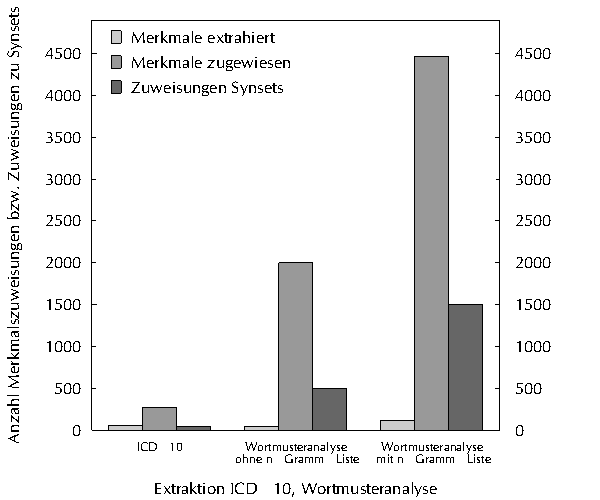
\includegraphics[width=0.48\textwidth]{icd10_affixe}
\hfill
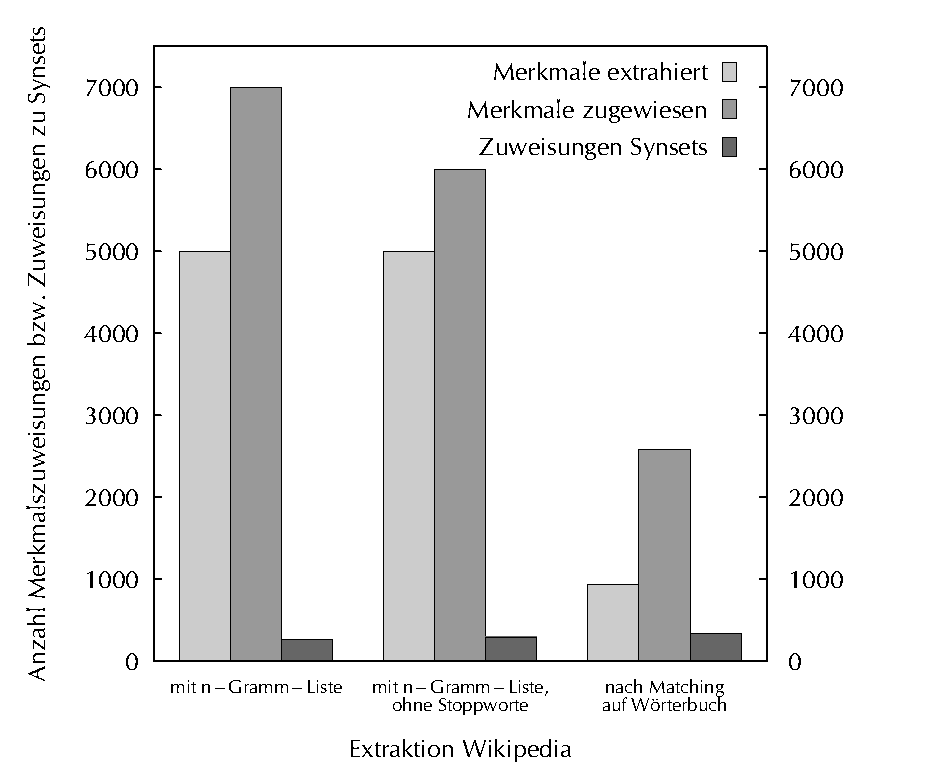
\includegraphics[width=0.48\textwidth]{wiki_extraktion}
\end{figure}

\section{Diskussion der Probleme}

Im Idealfall ist die Menge der verwendeten Merkmale genau so groß, wie sie sein muss, um alle formalen Begriffe bilden zu können und kein weiteres Merkmal zusätzlich. 
Insbesondere für allgemeine Übersetzungsaufgaben scheint es kaum vorstellbar eine Merkmalsmenge auf die hier vorgestellte Art zu verkleinern, ohne manuelle Korrekturen vorzunehmen. 
Bei der Beschränkung auf eine Domäne, so unsere initiale Annahme, müsste aber die automatisiert gewonnene Merkmalsmenge klein zu halten sein und dennoch ausreichend Zuweisungen erlauben. 
Aus unserer Sicht gab es vor allem zwei Problemstellen. 
\begin{enumerate}
\item Die Überdeckung der Wikipedia-Artikel mit den Einträgen des Wörterbuchs der Augenheilkunde. 
Je mehr Artikel aus der Wikipedia zu Einträgen aus dem Wörterbuch sich finden lassen, desto mehr unmittelbar passende Merkmale lassen sich aus den Artikeln extrahieren. 
\item Die Anzahl der unmittelbaren Übereinstimmungen in den Begriffen zwischen beiden betrug aber nur 335 Artikel-Eintrag-Kombinationen. 
%%%%%%%%%%%%%%%%%%%%%%%%%%%%%%%%%%%%%%%%%%%%%%%%%%%%%%%%%%%%%%%%%%%%%%%%%%%%%%%%
%% TODO '335 Artikel-Eintrag-Kombinationen': wieviele Artikel wurden dafür herangezogen, wieviele Einträge?
%%%%%%%%%%%%%%%%%%%%%%%%%%%%%%%%%%%%%%%%%%%%%%%%%%%%%%%%%%%%%%%%%%%%%%%%%%%%%%%%
Weil die Anzahl der Artikel in der englischsprachigen Wikipedia maximal ist (absolut, aber auch unterhalb der Kategorie \emph{Ophthalmology}, verwendeten wir die Einträge daraus. 
Da die Auswahl geeigneter Merkmale im Wesentlichen einer Verschlagwortung der untersuchten Domäne gleichkommt, wurden unsere Ergebnisse auch besser, je mehr typische Schritte zur Schlagwortgewinnung wir durchführten (Stemming, Zerlegen in n-Gramme). 
\end{enumerate}

\section{Auf diese Arbeit aufbauende weitere Ansätze}
\subsection{Evaluation durch Einschränkung der Merkmalsmenge}

Die Ergebnisse bezüglich der gewonnenen Menge an Merkmalen sind schwer zu beurteilen.
Die Menge der extrahierten Merkmale wurde nicht versucht zu verkleinern.
Sie besteht aus allen Worten, die in den einführenden Sätzen der Wikipedia-Artikel vorkamen und die nach den geschilderten Schritten, insbesondere Stemming, verblieben sind.
Mit steigender Zahl der Merkmale wird es schwieriger, kohärente Begriffsverbände zu erzeugen, weil zuviele Begriffe zu wenige gemeinsame Merkmale haben, oder nur solche von sehr allgemeiner Natur.
Eine Möglichkeit die Merkmalsmenge zu reduzieren und dieses Problem unmittelbar anzugehen ist zu versuchen Synonyme in der Merkmalsmenge zu identifizieren, einen der synonymischen Begriffe auszuwählen und alle anderen durch diesen zu ersetzen.
Dies könnte in Teilen mittels eines Wörterbuchs automatisch erledigt werden, weil viele Bezeichnungen der Merkmale entweder nicht spezifisch aus der Domäne der Augenheilkunde sind, sondern Teil der normalen Sprache, oder allgemeinere medizinische Bezeichnungen sind, für die es (beispielsweise ein englisches) Wörterbuch mit Synonymen gibt.
Dennoch: ein verbleibender Teil müsste vermutlich per Hand erledigt werden.
Mit dieser neuen Merkmalsmenge könnte man dann erneut versuchen Begriffsverbände zu bilden und Zuweisungen zu den Einträgen zu produzieren, um zu vergleichen, ob eine größere Zahl Zuweisungen erreicht wurde und ob die Anzahl gemeinsamer Merkmale gesteigert werden konnte.

Auf diesen Gedanken aufbauend, scheint es uns vielversprechend, mit Teilmengen unterschiedlicher Größe der ursprünglichen Merkmalsmenge zu experimentieren.
Den bei den 'echten' Synonymen verfolgten Ansatz könnte man hierzu erweitern und beispielsweise sämtliche Merkmale als Synonyme von einem aus 30, 50 oder 70 zuvor ausgewählten Merkmalen zu definieren.
Dem Grunde nach ist das eine Verschlagwortung mittels eines kontrollierten Vokabulars und man müsste sehr umsichtig sein, welche Bezeichnungen man unter einer Merkmalsbezeichnung zusammenfasst, um nicht Ungenauigkeiten oder sogar Fehler in den resultierenden Begriffsverbänden zu bekommen.
Am Beispiel anatomischer Lagebezeichungnen sei aber kurz illustriert, wie das vonstatten gehen könnte:

\subsection{Automatisierung der Merkmalszuweisung}
Hierfür möglichst allgemeine, aber dennoch spezifizierende Merkmale verwenden, welche Synsets nach Aspekten unterscheiden bzw. gruppieren, die sehr gehäuft in der Domäne der Augenheilkunde auftreten und in der Betrachtung eines Fachkundige Relevanz haben (zum Beispiel Krankheit, Organ, Behandlungsmethode, diabetisch, usw.) 
Gründe dafür sind:
\begin{itemize}
\item die automatisierte Merkmalsgenerierung ist problematisch, da oft viel Ballast zustande kommt (gerade bei Methoden, die auf die linguistische Verarbeitung von Texten abzielt)
\item die Relevanz der extrahierten Merkmale ist nicht immer gegeben (möchte man wirklich nach diesem Merkmal unterscheiden?)
\item je größer der Merkmalsraum, desto schwieriger ist es, diesen automatisiert mit Merkmalszuweisungen zu füllen, um einen aussagekräftigen formalen Kontext zu generieren
\item bei Erstellung des Merkmalraums mit intellektuellem Aufwand und mithilfe von Fachwissen hat man deutlich mehr Kontrolle über die Bildung des Begriffverbandes
\end{itemize}

\subsection{Die Systematisierte Nomenklatur der Medizin (SNOMED)}

\subsection{Verschiedenes}

\subsection{Schlussbemerkungen}

\chapter{Anhang}

\subsection{Beispiel für die Verarbeitung der Extrakte aus der Wikipedia}

Basierend auf den Kategorien, wurden alle Artikel, denen ein gegebenes Kategorie-Tag zugewiesen war geholt (genaueres, siehe XXX).

\lstset{
language=XML
}

\begin{lstlisting}
<?xml version="1.0"?>
<api>
<query>
<pages>
<page pageid="3055944" ns="0" title="Parinaud&#039;s syndrome">
<categories>
<cl ns="14" title="Category:Diseases of the eye and adnexa" />
<cl ns="14" title="Category:Medical signs" />
</categories>
<extract xml:space="preserve">
Parinauds Syndrome, also known as dorsal midbrain syndrome is a group of abnormalities of eye movement and pupil dysfunction.
</extract>
</page>
</pages>
</query>
</api>
\end{lstlisting}

Von Interesse sind hier der eigentliche Titel des Dokuments, die Kategorien und das Extrakt selbst. 
Die Kategorien wurden extrahiert, um hinterher kontrollieren zu können, dass alle Artikel geholt wurden (die Artikel wurden ja aufgrund ihrer Kategoriezugehörigkeit ausgewählt). 
Dabei gab es keine Abweichungen, der Schritt ist daher in Zukunft vermeidbar. 
Um den Titel in einem Ausdruck ohne das Markup zu holen, wurde folgender Ausdruck verwendet: 

\lstset{
language=bash
}

\begin{lstlisting}
sed -n 's/<page.*title="\([^"]*\)".*$/\1/p' Parinauds_syndrome.xml
\end{lstlisting}

Um das Extrakt in einem Ausdruck ohne das Markup zu holen, wurde
folgender Ausdruck verwendet:

\begin{lstlisting}
sed -n 's/<extract.*>\([^<]*\)\([<$ ].*\)/\1/p' Parinauds_syndrome.xml
\end{lstlisting}

HTML-Entities (wie \&\#39; für hochgestellte einzelne Anführungszeichen) wurden gesammelt und in der Ergebnisdatei in einem Durchgang ersetzt.
\end{document}
